\chapter{Einleitung}
\label{chapter:Einleitung}

Die Germanedge Solutions GmbH spezialisiert sich in der Digitalisierung der Produktion und
unterstützt Unternehmen mit individuellen Softwarelösungen für die Industrie 4.0 \cite{industry4dot0}.
Darunter auch ein nicht genannter Kunde, welcher Germanedge mit der Optimierung der Planung von Holzpressen beauftragt hat.
Dabei werden Holzbauteile zu Holzbalken verleimt und anschließend in Pressen gepresst.
Die Art und Weise der Anordnung der Bauteile in den Pressen wird als Pressenplan bezeichnet.
Abbildung \ref{figure:pressenplan} visualisiert einen solchen Pressenplan.
Die Presse (grau) presst in Richtung der Pfeile nach unten.
Die Balken (gelb) liegen horizontal und bestehen aus Bauteilen, welche durch die vertikalen (schwarzen) Linien getrennt sind.
Der Rest jedes Balkens ist rot hervorgehoben.

\begin{figure}[h]
    \centering
    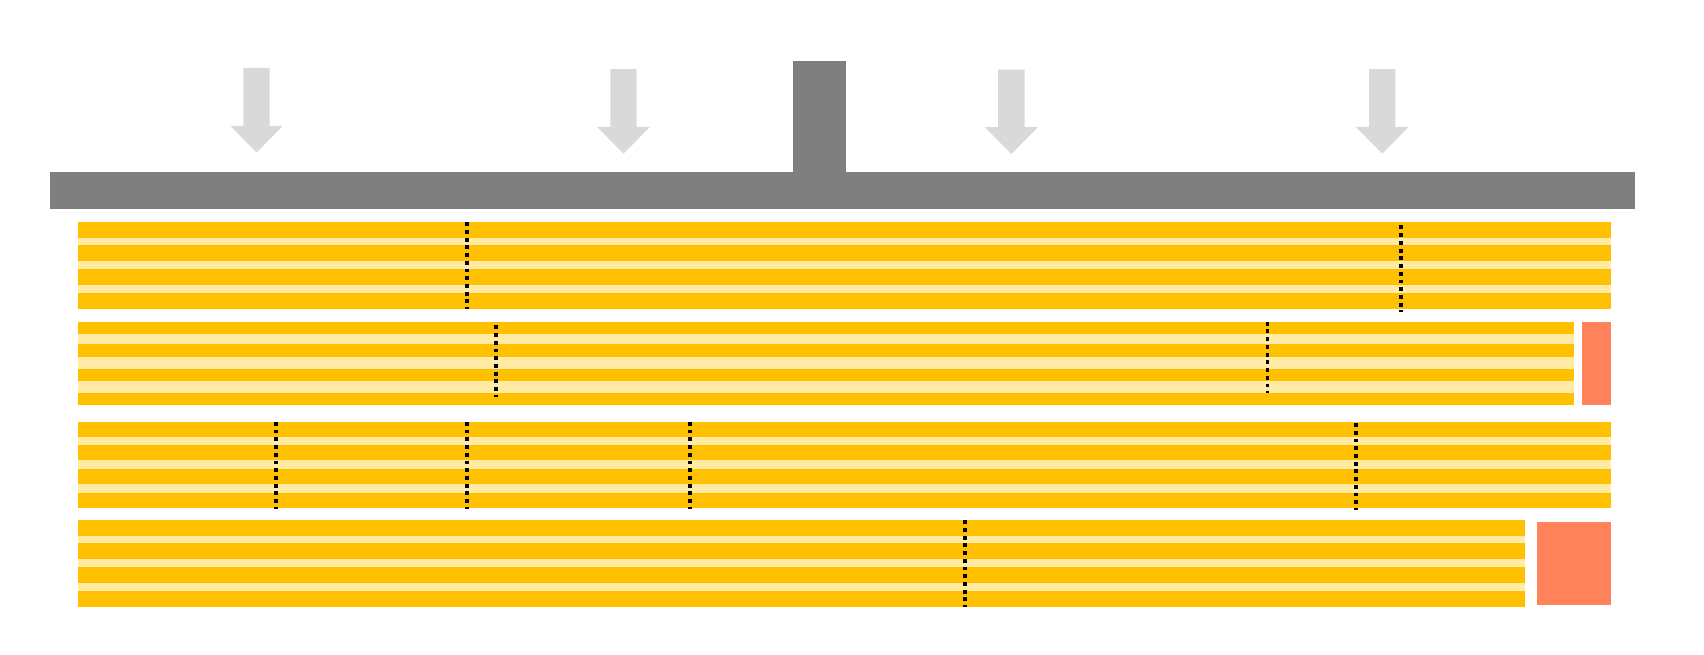
\includegraphics[width=1.00\textwidth, center]{Images/Pressenplan}\\
    \caption{Darstellung eines Pressenplans}
    \label{figure:pressenplan}
\end{figure}

An einen Pressenplan werden verschiedene Anforderungen wie beispielsweise die Gleichheit der Längen aller Balken in einer Presse gestellt.
Neben diesen Anforderungen sind auch einige Optimierungsziele für den Pressenplan von Bedeutung.
Darunter zum Beispiel die Minimierung des Rests, der Balken auf die gleiche Länge auffüllt und somit zusätzliche Materialkosten bedeutet.

Germanedge konnte für dieses Problem bereits eine Lösung finden, diese ist allerdings unter Firmenverschluss.
Es ist lediglich bekannt, dass jene einen heuristischen Ansatz wählt.
Das ermöglicht zwar einerseits das schnelle Ermitteln von Lösungen nahe am Optimum, andererseits gehen dabei aber auch (optimale) Lösungen verloren.

Daher wird in dieser Arbeit ein neuer, vollständiger Ansatz zur Lösung des Problems gewählt.
Dieser besteht in der Kodierung der Anforderungen an den Pressenplan als Constraints in einem Constraint-System.
Ein Constraint ist hier eine prädikatenlogische Formel, welche unter einer erfüllenden Belegung den Wahrheitswert \texttt{Wahr} haben muss.
Ein Constraint-System besteht aus der Konjunktion mehrerer Constraints.

In dieser Arbeit wird das Constraint-System für die Satisfiability Module Theories (kurz SMT) mithilfe des Sprachstandards SMTLib Version 2.6 \cite{smtlib} kodiert.
Zu typischen Anwendungsbereichen von SMT gehören neben der Programmverifikation \cite{smt} auch Ressourcenzuordnungsprobleme \cite{rcpsp,smartnocs}.
Das Pressenplanungsproblem kann als Ressourcenzuordnungsproblem betrachtet werden, sodass sich die Frage stellt, wie es als SMT-Problem in SMTLib kodiert werden kann.
Eine Beispieleingabe von Bauteilen könnte folgende sein:

\begin{table}[H]
    \centering
    \begin{tabular}{|c|c|c|}
        \hline
        \textbf{Länge in mm} & \textbf{Höhe in mm} & \textbf{Anzahl} \\
        \hline
        7000 & 400 & 1 \\
        13000 & 400 & 2 \\
        3000 & 400 & 3 \\
        6000 & 400 & 1 \\
        9000 & 400 & 1 \\
        7500 & 400 & 1 \\
        5000 & 400 & 1 \\
        5500 & 400 & 1 \\
        3500 & 400 & 1 \\
        \hline
    \end{tabular}
    \caption{Beispieleingabe von Bauteilen, jede Zeile entpricht einer Bauteilspezifikation}
    \label{table:bauteileingabe}
\end{table}

Da das Formulieren der Constraints für einen Pressenplan mit gegebenen Bauteilen händisch in der Constraint-Sprache SMTLib sehr schwer- und fehleranfällig ist
(siehe Listing \ref{listing:barLengthSMTlib}), erzeugt ein Programm in einer Gastsprache das Constraint-System für die Constraint-Sprache.
Für diese Arbeit wird als jene Gastsprache Haskell \cite{haskellhistory} gewählt.
Mit der Haskell-Bibliothek \texttt{Hasmtlib} \cite{hasmtlib} lässt sich beispielhaft das bereits erwähnte Constraint
gleicher Länge aller Balken in einer Presse folgend formulieren:

\begin{listing}[H]
    \inputminted[linenos=true]{haskell}{Code/Einleitung/PressenlängeConstraintHaskell.hs}
    \caption{Haskell-Code für das Constraint: $ \forall \{b_1, b_2\} \in \binom{Balken}{2}: presse(b_1) = presse(b_2) \rightarrow l\ddot ange(b_1) = l\ddot ange(b_2) $}
    \label{listing:barLengthCode}
\end{listing}

Die Bibliothek erzeugt dann das Constraint-System in der Constraint-Sprache SMTLib.
Folgend ein Ausschnitt der erzeugten SMTLib-Kodierung für das Constraint aus Listing \ref{listing:barLengthCode}:

\begin{listing}[H]
    \inputminted{bash}{Code/Einleitung/PressenlängeConstraintSMTLib.smt2}
    \caption{Ausschnitt der Kodierung eines Pressenplanungsproblems}
    \label{listing:barLengthSMTlib}
\end{listing}

Die Kodierung wird an einen SMT-Solver gegeben, welcher die Erfüllbarkeit des Problems bestimmt und für den Fall \textit{erfüllbar} eine erfüllende Belegung für die Variablen des Problems ermittelt.
Zum Beispiel:

\begin{listing}[H]
    \inputminted[linenos=true]{bash}{Code/Einleitung/PressenlängeConstraintSolverOutput.smt2}
    \caption{Ausschnitt des Solver-Outputs der Lösung eines Pressenplanungsproblems}
    \label{listing:barLengthSolverOutput}
\end{listing}

Jene Belegung transformiert das Programm dann in das gewünschte Ausgabeformat:

\begin{table}[H]
    \centering
    \begin{tabular}{|c|c|c|c|c|}
        \hline
        \textbf{Presse} & \textbf{Schicht} & \textbf{Position} & \textbf{Länge in mm} & \textbf{Höhe in mm} \\
        \hline
        1 & 1 & 1 & 14000 & 400 \\
        1 & 1 & 2 & 7500 & 400 \\
        1 & 2 & 1 & 3000 & 400 \\
        1 & 2 & 2 & 6500 & 400 \\
        1 & 2 & 3 & 3000 & 400 \\
        \ldots & \ldots & \ldots & \ldots & \ldots \\
        \hline
    \end{tabular}
    \caption{Beispielausgabe des Pressenplans, Visualisierung in Abbildung \ref{figure:pressenplan}}
    \label{table:pressenplan}
\end{table}

% TODO: Waldmann sagt: Bestenfalls nicht hier hinten dran schmeißen, sondern in Einleitungstext integrieren

Die Struktur dieser Arbeit ist folgende:

in Kapitel \ref{chapter:problem} wird das Problem der Pressenplanung erklärt, modelliert und nach, für das Problem relevanten, Zielfunktionen optimiert.

Folgend wird in Kapitel \ref{chapter:smt} gezeigt, wie Erfüllbarkeitsprobleme der Satisfiability Modulo Theories im Sprachstandard SMTLib Version 2.6 kodiert werden können.

In Kapitel \ref{chapter:haskell} wird auf einige notwendige Grundlagen von Haskell und die Haskell-Bibliothek \texttt{Hasmtlib} eingegangen.
Zusätzlich werden dort einige Erweiterungen von \texttt{Hasmtlib} diskutiert.

Danach wird die Kodierung des in Abschnitt \ref{sec:modellierung} erstellten Modells des Pressenplanungsproblems mithilfe von \texttt{Hasmtlib}
in Kapitel \ref{chapter:implementierung} erläutert.

Weiter wird die Performance der Kodierung in Kapitel \ref{chapter:auswertung} mithilfe von Laufzeitmessungen ausgewertet und mit der bereits existenten Heuristik verglichen.

Abschließend wird das Ergebnis dieser Arbeit in Kapitel \ref{chapter:zusammenfassung} zusammengefasst.